\documentclass[draft]{homework}

\usepackage{fixme}
\usepackage{graphicx}
\usepackage{minted}
\usepackage{xspace}

\newcommand{\opn}{OPNsense\xspace}
\newcommand{\suri}{Suricata\xspace}

% Drop boxes around everything, used to mask pygments errors
\renewcommand{\fcolorbox}[4][]{#4}


\title{Practical Network Defense - Lab 7}
\subtitle{\suri on ACME co.}
\author{Alessandro Serpi - 1647244}
\date{3 May 2019}


\begin{document}
    \maketitle
    \tableofcontents
    
    
    \pagebreak
    \section{Introduction}
    An intrusion prevention systems (IPS) is a device that monitors a network to identify malicious activities, log information about them, report them and attempt to block them.
    The IPS that comes with \opn is \suri, owned and supported by the Open Information Security Foundation (OISF), a non-profit foundation.
    
    In this laboratory, \suri is configured in both firewalls to block the majority of suspect or potentially undesired activities (such as the Tor protocol and connections to social networks) and auto-update itself.
    
    
    \section{IPS configuration}
    In \textit{System} $\triangleright$ \textit{Services} $\triangleright$ \textit{Intrusion detection} $\triangleright$ \textit{Administration}, section \textit{Settings}, tick \textit{Enabled} and \textit{IPS mode} and select all interfaces in the setting of the same name.
    
    In section \textit{Download}, tick all checkboxes and click \textit{Enable (drop filter)}. Then, download and update the rules clicking on the specific button.
    
    In section \textit{Rules}, verify that there are enabled rules.
    In order to increase performances, only the most prominent rules are enabled by default: \suri is a highly memory-consuming applicative, enabling all rules would greatly affect network latencies.
    
    In section \textit{Schedule}, set the rules to auto-update every day at midnight.
    Tick the checkbox, set \texttt{0} to \textit{Hours} and \textit{Minutes} and \texttt{*} to all others time-related settings.
    
    
    \section{Custom rule writing and description}
    \subsection{EICAR string}
    EICAR (European Institute for Computer Antivirus Research), together with CARO (Computer Antivirus Research Organization), developed the EICAR test file: a harmless string designed to test the integrity of security software.
    Compliant applications treat the string as malicious content; in this case, the IPS blocks unencrypted TCP and UDP packets that contain the string.
    
    \subsection{Rules}
    The rules are (ordered by \texttt{sid}):
    \inputminted[breaklines]{suricata.py:SuriLexer -x}{../pnd-lab7-es1/web/var/www/html/suricata/custom.rules}
    
    The protocol is written in red; it is UDP for the first rule, TCP for the second one.
    Since the UDP \texttt{pcap} file is less complex, the corresponding rule was created first.
    
    The right-facing arrow states that the packets are checked only in one direction.
    Since the rules are checked against every packet, irregardless of its origin or destination (addresses and ports are in blue), it is useless to specify a bidirectional check.
    
    Options are between parentheses.
    \texttt{msg} is the rule description.
    \texttt{content} states which byte sequence (vertical bars delimit a sequence of bytes in hexadecimal form) the payload must have.
    \texttt{flow} applies only to TCP packet exchanges; it specifies that the packet must belong to an already-established connection.
    \texttt{classtype} is the rule type; since a test class does not exist, it was chosen a generic type.
    \texttt{sid} is the signature id; it must be unique.
    \texttt{rev} is the signature version; since the rules have not been updated yet, it is 1.
    
    \subsection{Rule installation}
    Since \opn does not allow to add new rules, it is necessary to create a downloadable ruleset in a web server and manually insert the definition file into the appropriate folder in both firewalls.
    
    First, create the file \texttt{custom.rules} with the two rules for the EICAR string in directory \texttt{var/www/html/suricata} of host \texttt{web.pndeflab.edu}, the only web server in this laboratory.
    Then, add the ruleset \texttt{Custom/custom} manually inserting the file \texttt{custom.xml}:
    \inputminted{xml}{files/custom.xml}
    \noindent in the directory \texttt{/usr/local/opnsense/scripts/suricata/metadata/rules} of both firewalls.
    
    
    \section{Test of the rules}
    Testing was performed manually, opening a terminal in both firewalls and trying to send the EICAR string using \textit{netcat}.
    The default policies were momentarily changed to allowing all incoming packets to avoid false negatives.
    
    For TCP, the pair of commands was
    \begin{minted}{sh}
        nc -l 55555  # server
        echo "$EICAR_STRING" | nc $OTHER_FIREWALL 55555  # client
    \end{minted}
    For UDP is identical, except for the flag \mintinline{sh}{-u}.
    
    The packets were never received by the server because they were blocked by the client, as showed by the alerts.
    \begin{figure}[H]
        \centering
        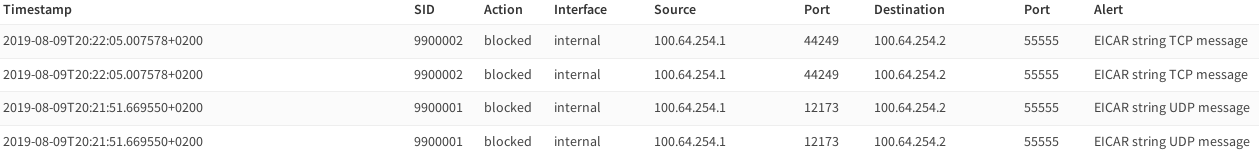
\includegraphics[width=\linewidth]{images/proof}
        \label{fig:proof}
    \end{figure}
    
    
    \section{Final remarks}
    \fxnote{TODO}
\end{document}
